%license:BSD-3-Clause
%copyright-holders:Michele Maione
%============================================================
%
%	Piattaforma di cloud gaming per giochi arcade
%
%============================================================
\chapter*{Ringraziamenti 2.0}

Ringrazio tutti coloro che hanno fatto parte del mio percorso di laurea magistrale:
\begin{itemize}
	\item la mia famiglia che crede sempre che io possa fare tutto, senza capire che nella mia limitatezza è sempre una faticaccia;	
	\item Laura Antonella (aka Dino) che con il suo amore ha chiuso il buco che avevo nel petto;
	\item Laura \& Giulia, Simona, Eleonora, Martina, Greta e tutte le altre ragazze del dipartimento di farmacia. Grazie per aver reso divertenti le giornate di studio. C'era sempre il sole in biblioteca;
	\item i miei giocatori del BawiTeam. Tra lacrime, infortuni, risate e gioie. Che squadra meravigliosa;
	\item i miei compagni di corso: Carrarini, Dettori, Iervolino, Lombardi, Bonapace, Paduano, Vannucci, Zhab'yak per i fantastici progetti fatti insieme;
	\item i professori del dipartimento di informatica. Ho cercato di trarre il massimo dai vostri insegnamenti per poterli poi concretamente utilizzare;
	\item Mario, Fede, Nadia, Giorgio, Giovanni e Mariapina per esserci sempre stati (da oltre 20 anni!);
	\item Alessandro, Carmen, Claudio, Sba, Marika, Grazia, Emiliana, Kikka, anche se non ci siamo visti spesso siete stati vicini;	
	\item i miei parenti di Treviglio che mi hanno aiutato e ospitato. Grazie per il supporto;
	\item tutti gli altri, anche se non menzionati, siete nel mio cuore.
\end{itemize}

Dedico questa tesi a Dino augurandole grandi successi accademici.

\begin{flushright}
	Milano, luglio 2021
\end{flushright}

\vspace*{\fill}

\begin{figure}[H]
	\centering
	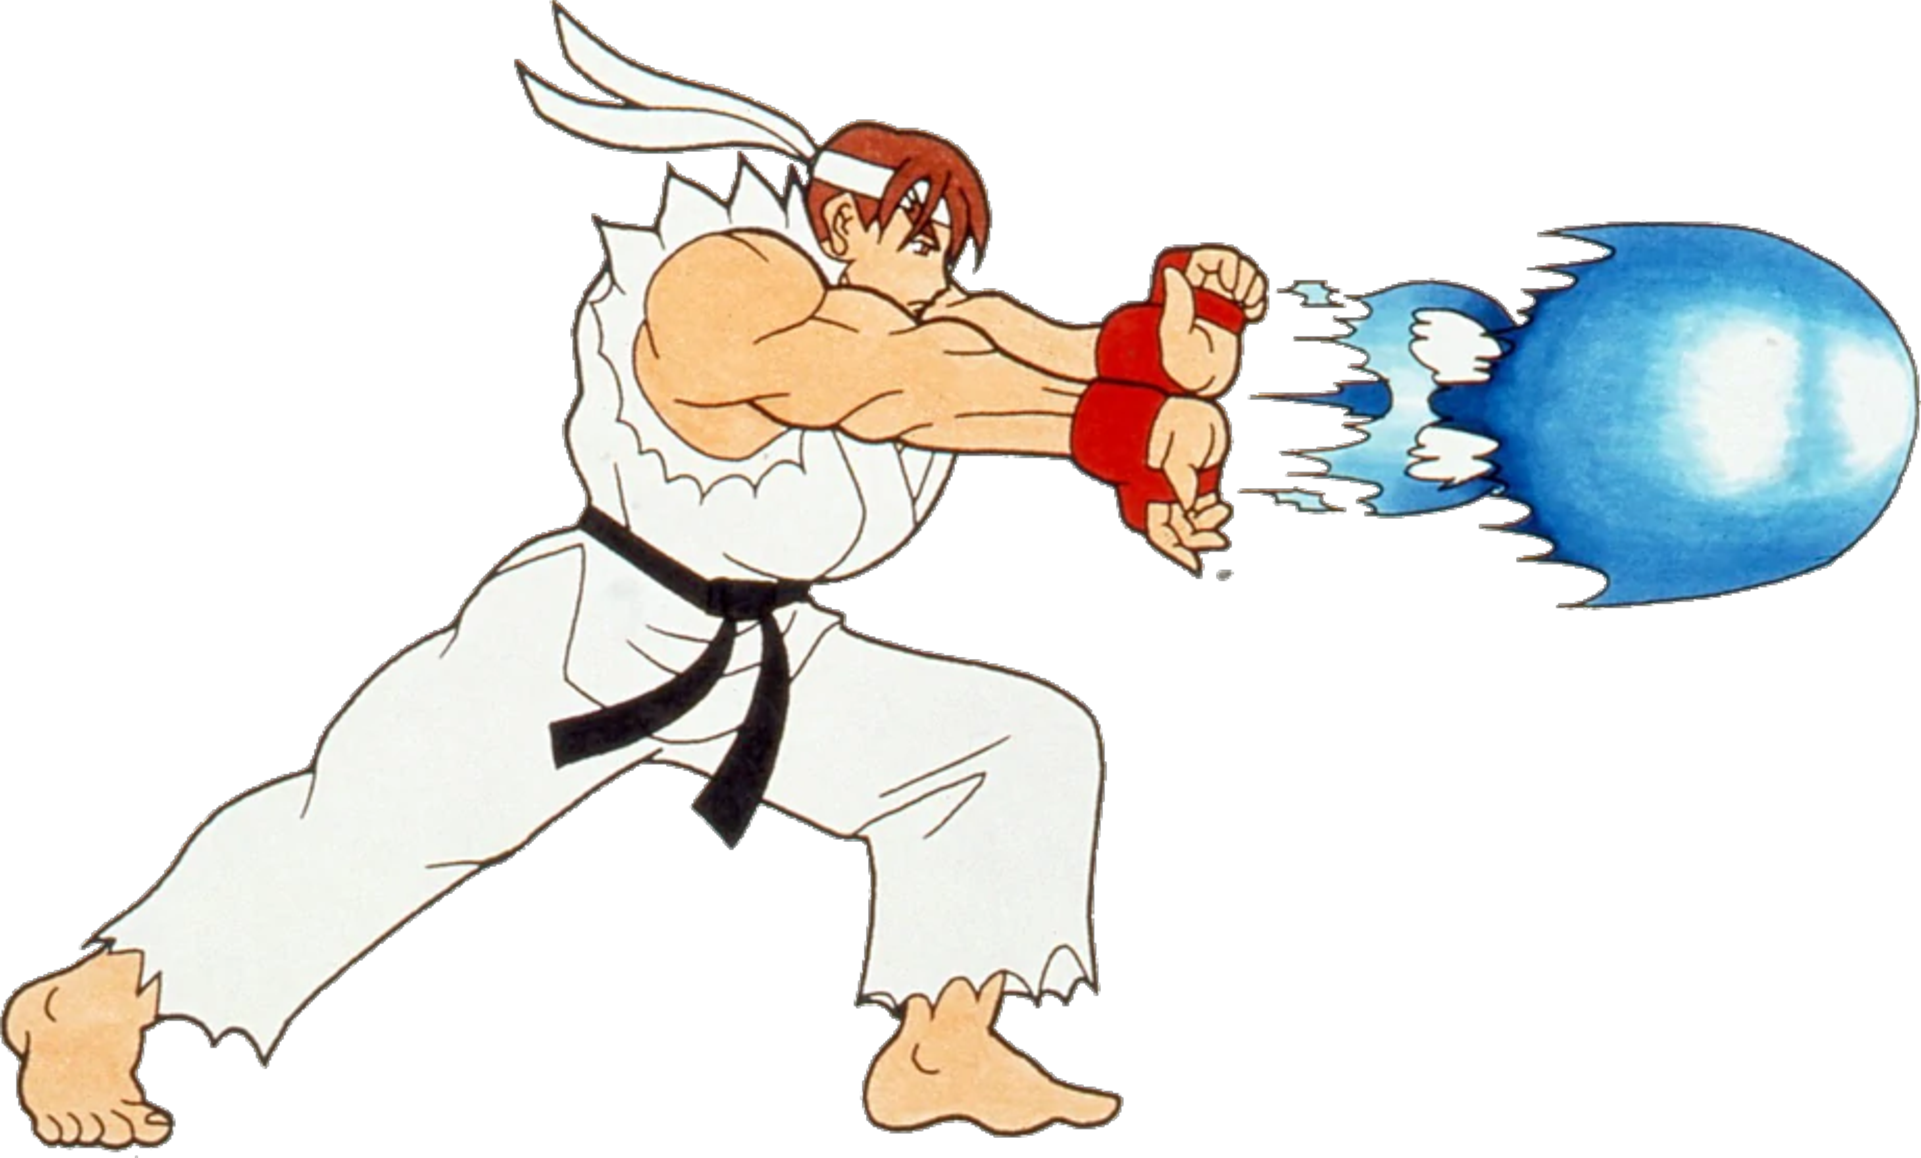
\includegraphics[width=5cm]{immagini/hadoken}
	\caption{Street Fighter Alpha artwork. © Capcom}
	\label{fig:hadoken}
\end{figure}